\begin{frame}[t]{Conclusão}
	Para efeitos de comparação, fizemos um teste da mesma função para os três métodos, e os resultados foram os seguintes:
	
\begin{figure}
	\centering
	\begin{minipage}{0.32\textwidth}
		\centering
		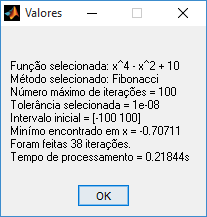
\includegraphics[width=3.5cm]{testfibo}
		\caption{Fibonacci}
		\label{fig:test_fibo}
	\end{minipage}\hfill
	\begin{minipage}{0.32\textwidth}
		\centering
		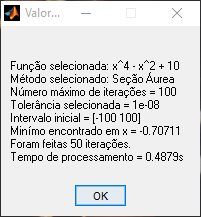
\includegraphics[width=3.5cm]{testaurea}
		\caption{Áurea}
		\label{fig:test_aurea}
	\end{minipage}
	\begin{minipage}{0.32\textwidth}
		\centering
		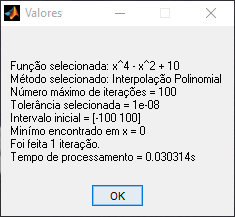
\includegraphics[width=3.5cm]{testinter}
		\caption{Interpolação}
		\label{fig:test_inter}
	\end{minipage}	
\end{figure}
	
\end{frame}

\begin{frame}[t]{Conclusão}
\begin{itemize}


	\item O método de interpolação polinomial chega ao mínimo \textbf{mais rapidamente}, porém apresenta \textbf{problemas de convergência} para funções não polinomiais.\\
	\vspace{2mm}
	\item Já os métodos de Fibonacci e Seção Áurea demoram um pouco mais para chegar a um resultado mas \textbf{convergem para uma vasta gama de funções}. De modo geral, o Fibonacci apresentou menor tempo de processamento do que a Seção Áurea.
	\end{itemize}
	
\end{frame}
